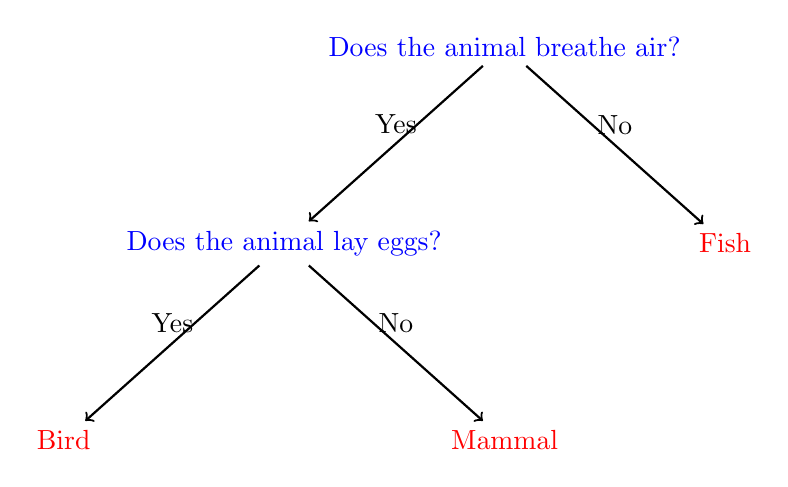
\begin{tikzpicture}[xscale = 2.8, yscale=2.5]
  \node (N1) at (0, 0) {
    \textcolor{blue}{Does the animal breathe air?}
  };

  \node (N2) at (-1, -1) {
    \textcolor{blue}{Does the animal lay eggs?}
  };

  \node (C1) at (-2, -2) {
    \textcolor{red}{Bird}
  };

  \node (C2) at (0, -2) {
    \textcolor{red}{Mammal}
  };

  \node (C3) at (1, -1) {
    \textcolor{red}{Fish}
  };

  \draw[thick, ->] (N1) -- (N2) node[midway, above] {Yes};
  \draw[thick, ->] (N2) -- (C1) node[midway, above] {Yes};
  \draw[thick, ->] (N2) -- (C2) node[midway, above] {No};
  \draw[thick, ->] (N1) -- (C3) node[midway, above] {No};
\end{tikzpicture}
